\documentclass[conference]{IEEEtran}
\IEEEoverridecommandlockouts
% The preceding line is only needed to identify funding in the first footnote. If that is unneeded, please comment it out.
\usepackage{cite}
\usepackage{amsmath,amssymb,amsfonts}
\usepackage{algorithmic}
\usepackage{graphicx}
\usepackage{textcomp}
\usepackage{xcolor}
\def\BibTeX{{\rm B\kern-.05em{\sc i\kern-.025em b}\kern-.08em
    T\kern-.1667em\lower.7ex\hbox{E}\kern-.125emX}}
\begin{document}

\title{Sistemi e Architetture per Big Data - AA 2020/2021 \\
	\LARGE \emph{Primo progetto}}

\author{\IEEEauthorblockN{Giuseppe Lasco}
\IEEEauthorblockA{\textit{Dipartimento di Ingegneria dell'Informazione} \\
\textit{Universit\`{a} degli studi di Roma "Tor Vergata"
}\\
Roma, Italia \\
giuseppe.lasco17@gmail.com}
\and
\IEEEauthorblockN{Marco Marcucci}
\IEEEauthorblockA{\textit{Dipartimento di Ingegneria dell'Informazione} \\
\textit{Universit\`{a} degli studi di Roma "Tor Vergata"
}\\
Roma, Italia \\
marco.marcucci96@gmail.com}

}

\maketitle

\begin{abstract}
Questo documento riporta i dettagli implementativi
riguardanti l'analisi mediante \emph{Spark} dei dataset contenenti
informazioni relative all'andamento nazionale italiano dei
vaccini effettuati. Viene, inoltre, descritta l'architettura 
a supporto dell'analisi e gli
ulteriori ​\emph{framework}​ utilizzati.
\end{abstract}

\section{\textbf{Introduzione}}
L'analisi effettuata si pone lo scopo di valutare delle
statistiche relative ai vaccini contro il COVID-19, su dati 
resi disponibili dal Commissario straordinario per l'semergenza Covid-19, 
Presidenza del Consiglio dei Ministri.\\
\subsection*{\textbf{Dataset}} 
Il primo file preso in considerazione \`{e} \textit{punti-somministrazione-tipologia.csv}, il quale contiene dati sui punti di somministrazione per ciascuna Regione e Provincia Autonoma.
\par Il secondo file preso in considerazione \`{e} \textit{somministrazioni-vaccini-latest.csv}, il quale contiene dati sulle somministrazioni giornaliere dei vaccini suddivisi per regioni, fasce d’et\`{a} e categorie di appartenenza dei soggetti vaccinati. Tale dataset risulta ordinato per data,
inoltre \`{e} stata riscontrata l'assenza di numerose tuple relative a delle specifiche regioni, fasce d'eta\`{a} e mesi. Questo fenomeno ha reso necessario un intervento di preprocessamento utile a inserire date mancanti per rendere pi\`{u} accurato il lavoro di regressione sui dati, sotto l'assunzione che i dati mancanti fossero dovuti all'assenza di vaccinazioni in un determinato giorno. 
\par Il terzo file preso in considerazione \`{e} \textit{somministrazioni-vaccini-summary-latest.csv}, il quale contiene dati sul totale delle somministrazioni giornaliere per regioni e categorie di appartenenza dei soggetti vaccinati. Il dataset in questione risulta, invece, non ordinato, per cui
si \`{e} reso necessario un effort di preprocessamento al fine di ordinarlo. 
\par L'ultimo file preso in considerazione \`{e} \textit{totale-popolazione.csv}, che tiene traccia
della popolazione totale residente in una data Regione o Provincia Autonoma.
\subsection*{\textbf{Query}}
L'obiettivo di questo progetto \`{e} quello di implementare ed eseguire tre query utilizzando \emph{Spark}.
\par La prima query ha come scopo quello di calcolare il numero medio di vaccinazioni giornaliere
in ciascun centro di ciascuna area.
\par La seconda consiste nel determinare le prime 5 aree per le quali è previsto il maggior numero di
vaccinazioni il primo giorno del mese successivo per le donne, per ogni fascia anagrafica e per ogni mese solare. A tale scopo si utilizza una retta di regressione, addestrata sui dati relativi al mese
precedente a quello per cui viene fatta la predizione al primo giorno. I dati presi in considerazione partono dal 1 Febbraio 2021.
\par L'ultima query prevede di effettuare una previsione della percentuale totale delle somministrazioni dei vaccini al 1 Giugno 2021 per ogni regione, utilizzando tutti i dati relativi ai mesi precedenti, a partire dal 27 Dicembre 2020. Inoltre, vengono utilizzati due algoritmi di
clustering in grado di raggruppare le Regioni in base alla previsione sopra citata.
\subsection*{\textbf{Framework}}
Il progetto prevede l'utilizzo di alcuni \emph{framework} che permettono di rendere la computazione parallela e distribuita.
Come \emph{framework} di processamento batch \`{e} stato utilizzato \emph{Apache Spark} che comunica con
 lo storage distribuito \emph{Hadoop Distributed File System}. Per la raccolta dei risultati \`{e} stato impiegato \emph{HBase}, uno storage No-SQL column family. Infine, come \emph{framework} di data ingestion \`{e} stato utilizzato \emph{NiFi}.
\section{\textbf{Architettura}}
L'architettura si compone di un insieme di container \emph{Docker}, su cui eseguono i servizi introdotti precedentemente. Inoltre, sempre sulla stessa macchina, una JVM ospita l'esecuzione di \emph{Apache Spark}. I container comunicano attraverso la stessa rete, creata appositamente.
\begin{figure}[htbp]
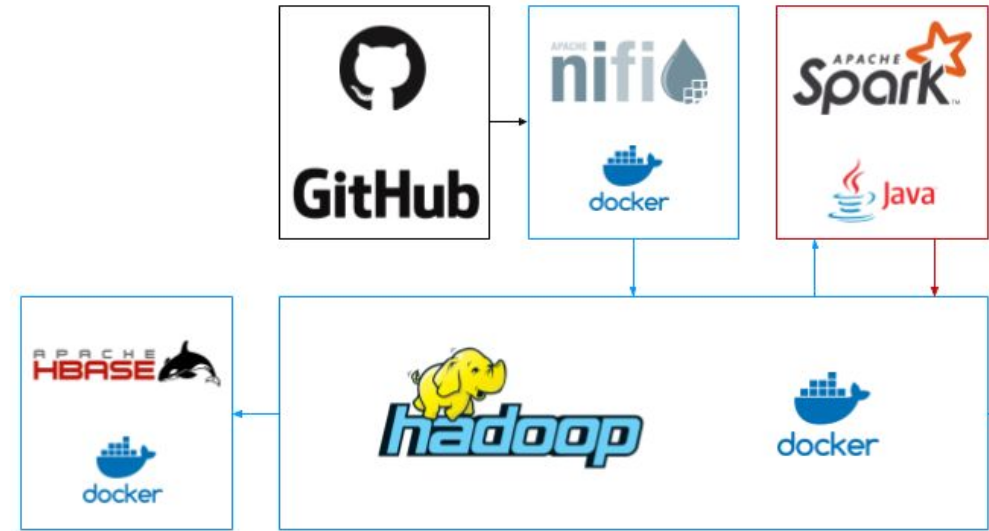
\includegraphics[scale=0.24]{frameworks.png}
\caption{Schema dell'architettura}\label{figura:architettura}
\label{fig}
\end{figure}

\subsection*{\textbf{NiFi}}
\emph{NiFi} \`{e} il servizio che permette di recuperare i dataset in formato \emph{comma separated value} da \emph{GitHub}, trasformarli in formato \emph{parquet} e inviarli al servizio di storage distribuito \emph{HDFS}. Tale \emph{framework} \`{e} stato istanziato su container \emph{Docker} utilizzando l'immagine \emph{apache/nifi}.
L'uso di \emph{parquet} ha permesso di comprimere i dati migliorando le prestazioni in termini di occupazione di memoria. \textbf{***colonne***}
\par Al fine di eseguire le operazioni elencate, sono stati impiegati due \emph{processori}, uno che permette di collegarsi al servizio di hosting \emph{GitHub} e scaricare i dati e uno che permette la trasformazione in \emph{parquet} di questi ultimi e l'upload su \emph{HDFS}. La struttura \`{e} definita mediante il template in figura ~\ref{figura:template}.
\begin{figure}[htbp]
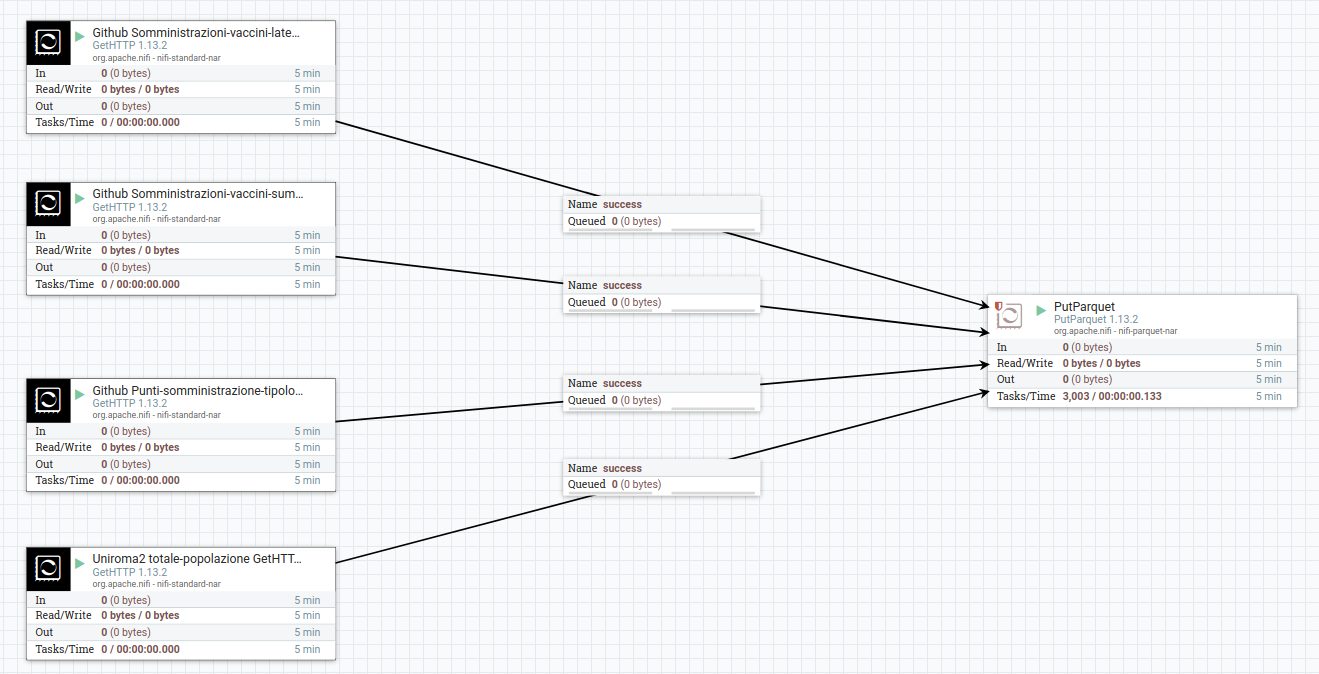
\includegraphics[scale=0.19]{NiFi_template.png}
\caption{NiFi template}\label{figura:template}
\label{fig}
\end{figure}

\subsection*{\textbf{HDFS}}
\emph{HDFS} rappresenta il mezzo che permette l'archiviazione dei dati in maniera distribuita. Il servizio si compone di un nodo \emph{master} e tre nodi \emph{worker} con un livello di replicazione pari a 2. Tale servizio permette di rendere disponibili i dati su cui \emph{Spark} esegue la computazione e memorizza gli \emph{output} dell'analisi, che vengono, in seguito, esportati su \emph{HBase}, per eventuali analisi, manipolazione e rappresentazione dei dati. Il deployment del framework avviene attraverso l'utilizzo dell'immagine \emph{Docker} \emph{effeerre/hadoop}, istanziata su container. In seguito all'avvio del servizio, uno script permette di eseguire lo sturtup del \emph{Namenode} e dei \emph{Datanode}, e crea le directory \texttt{/data}, dove \emph{NiFi} inserisce i dati, e \texttt{/output}, in cui risiedono i risultati dell'analisi, concedendo i permessi di lettura, scrittura ed esecuzione.

\subsection*{\textbf{Spark}}
Al fine di preocessare i dati ed eseguire le \emph{query}, viene utilizzato \emph{Apache Spark} in locale, tramite lo script \texttt{\$SPARK\_HOME/bin/spark-submit}. Oltre allo \emph{Spark Core}, che espone un set di API di \emph{trasformazioni} ed \emph{azioni}, \`{e} stata impiegata la libreria di \emph{Machine Learning} \emph{MLlib}, utile per effettuare \emph{clustering} sui risultati della terza \emph{query}. 

\subsection*{\textbf{HBase}}
Hbase \`{e} stato utilizzato come datastore \emph{NoSQL} sul quale
importare i risultati delle ​query,​ anche questo servizio \`{e}
stato istanziato utilizzando un ​container \emph{Docker} realizzato,
questa volta, a partire dall'immagine​ \emph{harisekhon/hbase}​. Affinch\`{e} fosse possibile
l'esportazione dei risultati da \emph{HDFS} a \emph{HBase}, \`{e} stata creata la classe \texttt{HBaseQueries.java} che permette la creazione delle tabelle e l'inserimento dei dati, sfruttando la classe \texttt{HBaseClient.java}. Quest'ultima contiene informazioni riguardo la configurazione di \emph{HBase} e \emph{Zookeeper}, e le principali operazioni di gestione del datastore.\\\begin{list}{0}{\textbf{Lista:}}
\item  ewf
\item ef
\end{list}
\section{\textbf{Query}}
\subsection*{\textbf{Query 1}}
Al fine di soddisfare la seguente \emph{query}, si \`{e} reso necessario l'utilizzo di due file, \textit{somministrazioni-vaccini-summary-latest.parquet} e \textit{punti-somministrazione-tipologia.parquet}.\par
Tali file sono stati caricati in \texttt{Dataset} e trasformati in \texttt{JavaPairRDD}, considerando le sole colonne di interesse: \emph{data\_somministrazione}, \emph{area} e \emph{totale} per il primo e \emph{area} per il secondo.\par \`{E} stato effettuato un'ordinamento dell'\texttt{RDD} \textit{somministrazioni-vaccini-summary-latest} in base alla data, scartando i dati precedenti al 1 Gennaio 2021 e successivi al 31 Maggio 2021, utilizzando la \emph{trasformazione} di \emph{filter}. Un'\emph{azione} di \emph{reduceByKey} ha permesso di ottenere il totale di vaccinazioni per ogni mese. Utilizzando un approccio simile al \emph{word count}, sono stati contati i centri riferiti ad una determinata Regione relativi all'\texttt{RDD} \textit{punti-somministrazione-tipologia}. La \emph{join} ha permesso di unire i due \texttt{RDD}, utilizzando come chiave la Regione. Il risultato finale \`{e} stato ottenuto dividendo il totale per il numero di giorni del mese di riferimento e per il numero di centri della regione di riferimento, ordinando, infine, il risultato in termini di mese e regione.

\subsection*{\textbf{Query 2}}
Relativamente alla seconda \emph{query} \`{e} stato utilizzato il file \textit{somministrazioni-vaccini-latest.parquet}, il quale, in seguito al caricamento da \emph{HDFS}, \`{e} stato trasformato in \texttt{JavaPairRDD}. Durante questa fase sono state scartate le colonne irrilevanti ai fini della richiesta. La \emph{trasformazione "filter"} ha permesso l'eliminazione delle entry relative a date precedenti al 1 Febbraio 2021 e successivi al 1 Giugno 2021. Considerando come chiave la tupla \emph{area, data e fascia anagrafica} sono stati sommati i vaccini relativi ad aziende farmaceutiche differenti. La \emph{trasformazione "groupByKey"} \`{e} stata applicata al fine di raggruppare tutte le tuple \emph{data, numero somministrazioni giornaliere} relative ad una certa regione e fascia anagrafica. Per ogni mese \`{e} stato eseguito una operazione di inserimento di date e valori macanti ed \`{e} stata effettuata \emph{regressione lineare} per ogni mese, in modo da prevedere il numero di donne vaccinate al primo giorno del mese successivo. Il modello di regressione lineare \'{e} stato addestrato attraverso l'implementazione fornita dalla libreria di regressione di \texttt{Apache Commons}.

\subsection*{\textbf{Query 3}}
L'ultima \emph{query} fa uso dei dati presenti nei file \textit{somministrazioni-vaccini-summary-latest.parquet} e \textit{totale-popolazione.parquet}. In seguito si \`{e} passati al caricamento dei file e alla trasformazione in \texttt{JavaPairRDD}. Sui dati relativi a \textit{somministrazioni-vaccini-summary-latest} si \`{e} proceduto al raggruppamento delle tuple \emph{data, numero somministrazioni giornaliere} per ogni regione, questa operazione ha permesso di svolgere regressione lineare su tutti i giorni dal 27 Dicembre 2020 al 31 Maggio 2021, in modo da prevedere il numero di vaccini effettuati in data 1 Giugno 2021. Una \emph{reduceByKey} sulle regioni ha, invece, permesso di calcolare il totale di vaccini effettuati dal 27 Dicembre 2020 al 31 Maggio 2021. Infine, l'operazione di somma tra le proiezioni e il totale calcolato, ha decretato il numero totale previsto di vaccinati per regione al 1 Giugno 2021. Il \emph{join} tra l'\emph{RDD} in questione e quello contenente il numero totale di abitanti residenti in ciacuna regione, he reso possibile clcolare la percentuale prevista di vaccinati al 1 Giugno 2021. Utilizzando due algoritmi presenti in \emph{MLLib}, \`{e} stato effettuato \emph{clustering} utilizzando i risultati precedenti come dataset, con numero di cluster variabile da 2 a 5. Gli algoritmi utilizzati sono \emph{K-means} e \emph{Bisecting K-means}, mentre per la regressione \`{e} stata utilizzata l'implementazione fornita dalla libreria di regressione di \texttt{Apache Commons}.

\section{\textbf{Benchmark}}
L'esecuzione del progetto e la valutazione delle prestazioni sono state eseguite su Linux Mint 19.3 Cinnamon, Intel Core i7-8750H CPU, 6 core, 12 thread e 32 GB di RAM, con archiviazione su HDD. \\
\par In tabella~\ref{tab1} sono riportati i tempi di processamento delle query. Sono stati considerate le performance di puro processamento, ovvero non considerando i tempi di sturtup della \emph{Java Virtual Machine} su cui \emph{Spark} opera, il caricamento dei file dall'\emph{HDFS} e la scrittura dei risultati. Come si pu\`{o} notare, la query 3 risulta molto pi\`{u} lenta delle altre due, che, invece, mostrano risultati comparabili. Tale evidenza \`{e} causata dall'inclusione, nel totale, dei tempi di addestramento degli algoritmi di \emph{clustering}, che possono essere osservati in tabella~\ref{tab2}.

\begin{table}[htbp]
\caption{Tempi esecuzione query}
\begin{center}
    \begin{tabular}{|c|c|c|}
    \hline
    \textbf{Query} & \textbf{Media} & \textbf{Varianza}  \\ \hline
    Query 1 & 11C & 22C  \\ \hline
    Query 2 & 9C & 19C \\ \hline
    Query 3 & 10C & 21C  \\
    \hline
    \end{tabular}
\label{tab1}
\end{center}
\end{table}


\begin{table}[htbp]
\caption{Tempi esecuzione clustering}
\begin{center}
\begin{tabular}{|c|c|c|c|c|}
\hline
\textbf{}&\multicolumn{4}{|c|}{\textbf{Modello}} \\ \hline
\textbf{Numero} & \multicolumn{2}{|c|}{\textbf{K-means}} & \multicolumn{2}{|c|}{\textbf{Bisecting K-means}} \\ \cline{2-5} 
\textbf{cluster} & \textbf{Media} & \textbf{Varianza} & \textbf{Media} & \textbf{Varianza} \\ \hline

\end{tabular}
\label{tab2}
\end{center}
\end{table}

\begin{table}[htbp]
\caption{Costo clustering}
\begin{center}
\begin{tabular}{|c|c|c|}
\hline
\textbf{Numero}&\multicolumn{2}{|c|}{\textbf{Modello}} \\ \cline{2-3}
\textbf{cluster} & \multicolumn{1}{|c|}{\textbf{K-means}} & \multicolumn{1}{|c|}{\textbf{Bisecting K-means}} \\ \hline

\end{tabular}
\label{tab3}
\end{center}
\end{table}

\section{Prepare Your Paper Before Styling}
Before you begin to format your paper, first write and save the content as a 
separate text file. Complete all content and organizational editing before 
formatting. Please note sections \ref{AA}--\ref{SCM} below for more information on 
proofreading, spelling and grammar.

Keep your text and graphic files separate until after the text has been 
formatted and styled. Do not number text heads---{\LaTeX} will do that 
for you.

\subsection{Abbreviations and Acronyms}\label{AA}
Define abbreviations and acronyms the first time they are used in the text, 
even after they have been defined in the abstract. Abbreviations such as 
IEEE, SI, MKS, CGS, ac, dc, and rms do not have to be defined. Do not use 
abbreviations in the title or heads unless they are unavoidable.

\subsection{Units}
\begin{itemize}
\item Use either SI (MKS) or CGS as primary units. (SI units are encouraged.) English units may be used as secondary units (in parentheses). An exception would be the use of English units as identifiers in trade, such as ``3.5-inch disk drive''.
\item Avoid combining SI and CGS units, such as current in amperes and magnetic field in oersteds. This often leads to confusion because equations do not balance dimensionally. If you must use mixed units, clearly state the units for each quantity that you use in an equation.
\item Do not mix complete spellings and abbreviations of units: ``Wb/m\textsuperscript{2}'' or ``webers per square meter'', not ``webers/m\textsuperscript{2}''. Spell out units when they appear in text: ``. . . a few henries'', not ``. . . a few H''.
\item Use a zero before decimal points: ``0.25'', not ``.25''. Use ``cm\textsuperscript{3}'', not ``cc''.)
\end{itemize}

\subsection{Equations}
Number equations consecutively. To make your 
equations more compact, you may use the solidus (~/~), the exp function, or 
appropriate exponents. Italicize Roman symbols for quantities and variables, 
but not Greek symbols. Use a long dash rather than a hyphen for a minus 
sign. Punctuate equations with commas or periods when they are part of a 
sentence, as in:
\begin{equation}
a+b=\gamma\label{eq}
\end{equation}

Be sure that the 
symbols in your equation have been defined before or immediately following 
the equation. Use ``\eqref{eq}'', not ``Eq.~\eqref{eq}'' or ``equation \eqref{eq}'', except at 
the beginning of a sentence: ``Equation \eqref{eq} is . . .''

\subsection{\LaTeX-Specific Advice}

Please use ``soft'' (e.g., \verb|\eqref{Eq}|) cross references instead
of ``hard'' references (e.g., \verb|(1)|). That will make it possible
to combine sections, add equations, or change the order of figures or
citations without having to go through the file line by line.

Please don't use the \verb|{eqnarray}| equation environment. Use
\verb|{align}| or \verb|{IEEEeqnarray}| instead. The \verb|{eqnarray}|
environment leaves unsightly spaces around relation symbols.

Please note that the \verb|{subequations}| environment in {\LaTeX}
will increment the main equation counter even when there are no
equation numbers displayed. If you forget that, you might write an
article in which the equation numbers skip from (17) to (20), causing
the copy editors to wonder if you've discovered a new method of
counting.

{\BibTeX} does not work by magic. It doesn't get the bibliographic
data from thin air but from .bib files. If you use {\BibTeX} to produce a
bibliography you must send the .bib files. 

{\LaTeX} can't read your mind. If you assign the same label to a
subsubsection and a table, you might find that Table I has been cross
referenced as Table IV-B3. 

{\LaTeX} does not have precognitive abilities. If you put a
\verb|\label| command before the command that updates the counter it's
supposed to be using, the label will pick up the last counter to be
cross referenced instead. In particular, a \verb|\label| command
should not go before the caption of a figure or a table.

Do not use \verb|\nonumber| inside the \verb|{array}| environment. It
will not stop equation numbers inside \verb|{array}| (there won't be
any anyway) and it might stop a wanted equation number in the
surrounding equation.

\subsection{Some Common Mistakes}\label{SCM}
\begin{itemize}
\item The word ``data'' is plural, not singular.
\item The subscript for the permeability of vacuum $\mu_{0}$, and other common scientific constants, is zero with subscript formatting, not a lowercase letter ``o''.
\item In American English, commas, semicolons, periods, question and exclamation marks are located within quotation marks only when a complete thought or name is cited, such as a title or full quotation. When quotation marks are used, instead of a bold or italic typeface, to highlight a word or phrase, punctuation should appear outside of the quotation marks. A parenthetical phrase or statement at the end of a sentence is punctuated outside of the closing parenthesis (like this). (A parenthetical sentence is punctuated within the parentheses.)
\item A graph within a graph is an ``inset'', not an ``insert''. The word alternatively is preferred to the word ``alternately'' (unless you really mean something that alternates).
\item Do not use the word ``essentially'' to mean ``approximately'' or ``effectively''.
\item In your paper title, if the words ``that uses'' can accurately replace the word ``using'', capitalize the ``u''; if not, keep using lower-cased.
\item Be aware of the different meanings of the homophones ``affect'' and ``effect'', ``complement'' and ``compliment'', ``discreet'' and ``discrete'', ``principal'' and ``principle''.
\item Do not confuse ``imply'' and ``infer''.
\item The prefix ``non'' is not a word; it should be joined to the word it modifies, usually without a hyphen.
\item There is no period after the ``et'' in the Latin abbreviation ``et al.''.
\item The abbreviation ``i.e.'' means ``that is'', and the abbreviation ``e.g.'' means ``for example''.
\end{itemize}
An excellent style manual for science writers is \cite{b7}.

\subsection{Authors and Affiliations}
\textbf{The class file is designed for, but not limited to, six authors.} A 
minimum of one author is required for all conference articles. Author names 
should be listed starting from left to right and then moving down to the 
next line. This is the author sequence that will be used in future citations 
and by indexing services. Names should not be listed in columns nor group by 
affiliation. Please keep your affiliations as succinct as possible (for 
example, do not differentiate among departments of the same organization).

\subsection{Identify the Headings}
Headings, or heads, are organizational devices that guide the reader through 
your paper. There are two types: component heads and text heads.

Component heads identify the different components of your paper and are not 
topically subordinate to each other. Examples include Acknowledgments and 
References and, for these, the correct style to use is ``Heading 5''. Use 
``figure caption'' for your Figure captions, and ``table head'' for your 
table title. Run-in heads, such as ``Abstract'', will require you to apply a 
style (in this case, italic) in addition to the style provided by the drop 
down menu to differentiate the head from the text.

Text heads organize the topics on a relational, hierarchical basis. For 
example, the paper title is the primary text head because all subsequent 
material relates and elaborates on this one topic. If there are two or more 
sub-topics, the next level head (uppercase Roman numerals) should be used 
and, conversely, if there are not at least two sub-topics, then no subheads 
should be introduced.

\subsection{Figures and Tables}
\paragraph{Positioning Figures and Tables} Place figures and tables at the top and 
bottom of columns. Avoid placing them in the middle of columns. Large 
figures and tables may span across both columns. Figure captions should be 
below the figures; table heads should appear above the tables. Insert 
figures and tables after they are cited in the text. Use the abbreviation 
``Fig.~\ref{fig}'', even at the beginning of a sentence.

\begin{table}[htbp]
\caption{Table Type Styles}
\begin{center}
\begin{tabular}{|c|c|c|c|}
\hline
\textbf{Table}&\multicolumn{3}{|c|}{\textbf{Table Column Head}} \\
\cline{2-4} 
\textbf{Head} & \textbf{\textit{Table column subhead}}& \textbf{\textit{Subhead}}& \textbf{\textit{Subhead}} \\
\hline
copy& More table copy$^{\mathrm{a}}$& &  \\
\hline
\multicolumn{4}{l}{$^{\mathrm{a}}$Sample of a Table footnote.}
\end{tabular}
\end{center}
\end{table}

\begin{figure}[htbp]
\centerline{
\includegraphics{fig1.png}}
\caption{Example of a figure caption.}
\label{fig}
\end{figure}

Figure Labels: Use 8 point Times New Roman for Figure labels. Use words 
rather than symbols or abbreviations when writing Figure axis labels to 
avoid confusing the reader. As an example, write the quantity 
``Magnetization'', or ``Magnetization, M'', not just ``M''. If including 
units in the label, present them within parentheses. Do not label axes only 
with units. In the example, write ``Magnetization (A/m)'' or ``Magnetization 
\{A[m(1)]\}'', not just ``A/m''. Do not label axes with a ratio of 
quantities and units. For example, write ``Temperature (K)'', not 
``Temperature/K''.

\section*{Acknowledgment}

The preferred spelling of the word ``acknowledgment'' in America is without 
an ``e'' after the ``g''. Avoid the stilted expression ``one of us (R. B. 
G.) thanks $\ldots$''. Instead, try ``R. B. G. thanks$\ldots$''. Put sponsor 
acknowledgments in the unnumbered footnote on the first page.

\section*{References}

Please number citations consecutively within brackets \cite{b1}. The 
sentence punctuation follows the bracket \cite{b2}. Refer simply to the reference 
number, as in \cite{b3}---do not use ``Ref. \cite{b3}'' or ``reference \cite{b3}'' except at 
the beginning of a sentence: ``Reference \cite{b3} was the first $\ldots$''

Number footnotes separately in superscripts. Place the actual footnote at 
the bottom of the column in which it was cited. Do not put footnotes in the 
abstract or reference list. Use letters for table footnotes.

Unless there are six authors or more give all authors' names; do not use 
``et al.''. Papers that have not been published, even if they have been 
submitted for publication, should be cited as ``unpublished'' \cite{b4}. Papers 
that have been accepted for publication should be cited as ``in press'' \cite{b5}. 
Capitalize only the first word in a paper title, except for proper nouns and 
element symbols.

For papers published in translation journals, please give the English 
citation first, followed by the original foreign-language citation \cite{b6}.

\begin{thebibliography}{00}
\bibitem{b1} G. Eason, B. Noble, and I. N. Sneddon, ``On certain integrals of Lipschitz-Hankel type involving products of Bessel functions,'' Phil. Trans. Roy. Soc. London, vol. A247, pp. 529--551, April 1955.
\bibitem{b2} J. Clerk Maxwell, A Treatise on Electricity and Magnetism, 3rd ed., vol. 2. Oxford: Clarendon, 1892, pp.68--73.
\bibitem{b3} I. S. Jacobs and C. P. Bean, ``Fine particles, thin films and exchange anisotropy,'' in Magnetism, vol. III, G. T. Rado and H. Suhl, Eds. New York: Academic, 1963, pp. 271--350.
\bibitem{b4} K. Elissa, ``Title of paper if known,'' unpublished.
\bibitem{b5} R. Nicole, ``Title of paper with only first word capitalized,'' J. Name Stand. Abbrev., in press.
\bibitem{b6} Y. Yorozu, M. Hirano, K. Oka, and Y. Tagawa, ``Electron spectroscopy studies on magneto-optical media and plastic substrate interface,'' IEEE Transl. J. Magn. Japan, vol. 2, pp. 740--741, August 1987 [Digests 9th Annual Conf. Magnetics Japan, p. 301, 1982].
\bibitem{b7} M. Young, The Technical Writer's Handbook. Mill Valley, CA: University Science, 1989.
\end{thebibliography}
\vspace{12pt}
\color{red}
IEEE conference templates contain guidance text for composing and formatting conference papers. Please ensure that all template text is removed from your conference paper prior to submission to the conference. Failure to remove the template text from your paper may result in your paper not being published.

\end{document}
